\documentclass[a4paper,12pt]{article}
\usepackage{amsmath}
\usepackage{amsfonts}
\usepackage{amssymb}
\usepackage{amsthm}
\usepackage{mathtools}
\usepackage[utf8]{inputenc}
\usepackage[a4paper, margin=2cm]{geometry}
\usepackage{hyperref}
\usepackage{calrsfs}
\usepackage{graphicx}
\usepackage{grffile}
\usepackage{float}
\usepackage{bm}
\usepackage{cite}
\usepackage{nicefrac}
\usepackage{chngcntr}

\counterwithin{figure}{section}

\theoremstyle{definition}
\newtheorem{question}{Question}[section]
\newtheorem{definition}{Definition}[section]

\hypersetup{
	colorlinks=true,
	linkcolor=blue,
	filecolor=magenta,
	urlcolor=cyan,
}

\numberwithin{equation}{section}

\setlength{\parindent}{0em}
\setlength{\parskip}{1em}
\renewcommand{\baselinestretch}{1.15}

\allowbreak

% Subjective Logic macros

\usepackage{calrsfs}

% Domain
\newcommand{\dom}[1]{\mathbb{#1}}

% Powerset
\newcommand{\powset}[1]{\mathcal{P}(\mathbb{#1})}

% Hyperdomain
\newcommand{\hdom}[1]{\mathcal{R}(\mathbb{#1})}

% Composite set
\newcommand{\compset}[1]{\mathcal{C}(\mathbb{#1})}

% Base rate distribution
\newcommand{\ad}[1]{\mathbf{a}_{#1}}
\newcommand{\ada}[2]{\mathbf{a}^{#1}_{#2}}
\newcommand{\adx}[2]{\mathbf{a}_{#1}(#2)}
\newcommand{\adax}[3]{\mathbf{a}^{#1}_{#2}(#3)}

% Belief mass distribution
\newcommand{\bmd}[1]{\mathbf{b}_{#1}}
\newcommand{\bmda}[2]{\mathbf{b}^{#1}_{#2}}
\newcommand{\bmdx}[2]{\mathbf{b}_{#1}(#2)}
\newcommand{\bmdax}[3]{\mathbf{b}^{#1}_{#2}(#3)}

% Uncertainty mass
\newcommand{\ux}[1]{u_{#1}}
\newcommand{\uax}[2]{u^{#1}_{#2}}

% Projected Probability
\newcommand{\ppa}[2]{\mathbf{P}^{#1}_{#2}}

% Opinion
\newcommand{\opi}[1]{\omega_{#1}}
\newcommand{\opia}[2]{\omega^{#1}_{#2}}

\newcommand{\qm}[1]{`#1'}

\usepackage{xcolor}
\definecolor{darkgreen}{rgb}{0.0, 0.2, 0.13}
\definecolor{forestgreen(web)}{rgb}{0.13, 0.55, 0.13}
\definecolor{green(html/cssgreen)}{rgb}{0.0, 0.5, 0.0}

\newcommand{\red}{\textcolor{red}{red}}
\newcommand{\green}{\textcolor{green(html/cssgreen)}{green}}
\newcommand{\blue}{\textcolor{blue}{blue}}

%opening
\title{Subjective Logic}
\author{José C. Oliveira}

\begin{document}

\maketitle

\section{Introduction}

One of the major goals of our research is to develop a quantitative logic for reasoning about belief in social networks. Subjective logic is a logic that may have the expressiveness that we look for improve our influence graph and the belief state of an agent.

Subjective logic extends probabilistic logic. In probabilistic logic, we can express the truth value of a proposition by a probability distribution over a domain with disjoint events or states and reason by the axioms of probability. When we have two states of a domain $\dom{X}$ and the probability of a state $x \in \dom{X}$ can be $P(x) = 0$ or $P(x) = 1$, we have binary logic. The expression $x \land y$ is expressed in probabilistic logic as $P(x \land y) = P(x)P(y)$. Probabilistic logic extends binary logic.

Subjective logic extends probabilistic logic by adding \emph{uncertainty} and \emph{subjectivity}. We can't express \emph{\qm{we don't know}} with probabilistic logic by a uniform distribution because it says that we know that the distribution over the domain is uniform. Subjective logic can express that \emph{uncertainty} about the distribution. The \emph{subjectivity} comes from the fact that we can assign an opinion about a proposition to an agent.

By the investigation we are doing about subjective logic, our main question is: Can we use subjective logic to improve our model of social networks? If yes, how?

This document is an introduction about subjective logic and it will present elementary definitions, the definition of opinion, and trust opinions. The main reference of this document is the book \emph{Subjective Logic: A Formalism for Reasoning Under Uncertainty} by Audun Jøsang.


%\begin{itemize}
%	\item Probabilistic logic.
%	
%	\item Subjective logic as probabilistic logic with uncertainty and subjectivity.
%	
%	\item Main question of this investigation: Can we use Subjective Logic to improve the model?
%	
%	\item Summary.
%\end{itemize}

\section{Opinion representation}

The main object of subjective logic is the \emph{opinion}, and there are many equivalent ways for opinion representation. Here I will present the most used one. We represent an opinion by $\opia{A}{X}$, where $A$ is an agent and $X$ is a random variable or a \emph{hypervariable}. This section presents the elementary definitions that compose an opinion.

\subsection{Elementary definitions}

\subsubsection{Domain and hyperdomain}

In subjective logic, a domain is a state space consisting of a set of values which can also be called states, events, outcomes, hypotheses or propositions. Those values are assumed to be exclusive and exhaustive. Let $k = |\dom{X}|$ be the cardinality of $\dom{X}$.

Suppose we have a box that has balls that can \red, \green, or \blue. Then the domain that represents all the outcomes is
\begin{equation}
	\dom{X} = \{\red, \green, \blue\}\text{.}
\end{equation}


\begin{definition}
	 \emph{(Hyperdomain)} Let $\dom{X}$ be a domain, and let $\powset{X}$ denote the powerset of $\dom{X}$. The powerset contains all subsets of $\dom{X}$, including the empty set $\emptyset$, and the domain $\dom{X}$ itself. The \emph{hyperdomain} denoted $\hdom{X}$ is the reduced powerset of $\dom{X}$, i.e. the powerset excluding the empty-set $\varnothing$ and the domain value $\dom{X}$. The hyperdomain is expressed as
	\begin{equation}
		\text{Hyperdomain:}\ \mathcal{R}(\mathbb{X}) = \mathcal{P} \setminus \{\mathbb{X}, \emptyset\}
	\end{equation}
\end{definition}

The hyperdomain of the box is
\begin{equation}
    \begin{array}{rll}
        \hdom{\dom{X}} = \{ & \{\red\}, \{\green\}, \{\blue\}, \\
        & \{\red, \green\}, \{\red, \blue\}, \{\green, \blue\} & \}\text{.}
    \end{array}
\end{equation}

Let $\kappa = |\hdom{X}| = 2^k -2\text{.}$ be the cardinality of $\hdom{R}$.

Every value of the hyperdomain with one value is called \emph{singleton}. Every value with more than one value is called \emph{composite value}. The interpretation of a composite value being TRUE, is that one and only one of the constituent singletons is TRUE. The set of all composite values $\compset{X}$ is called \emph{composite set}.

A \emph{hypervariable} $X$ is an random variable that takes its values from $\hdom{X}$. For example, if a hypervariable takes its values from the composite value $\{\blue, \red\} \in \hdom{X}$, it means that we either draw a ball \blue\ or \red.

\subsubsection{Belief mass distribution and uncertainty mass}

\emph{Belief mass} is distributed over a (hyper)domain. Assign belief mass to a singleton value $x \in \dom{X}$ expresses support for $x$ being TRUE. Assign belief mass to a composite value $x \in \compset{X}$ express support for one of the singleton values in $x$ being TRUE. Belief mass is sub-additive and is complemented by \emph{uncertainty mass} $\ux{X}$ and it represents vacuity of evidence, i.e. the lack of support for the variable $X$ to have any specific value.

\begin{definition}
	\emph{(Belief Mass Distribution)} Let $\mathbb{X}$ be a domain with corresponding hyperdomain $\mathcal{R}(\mathbb{X})$, and let $X$ be a variable over those domains. A belief mass distribution denote $\mathbf{b}_X$ assigns belief mass to possible values of the variable $X$. In the case of a random variable $X \in \mathbb{X}$, the belief mass distribution applies to domain $\mathbb{X}$, and in the case of a hypervariable $X \in \mathcal{R}(\mathbb{X})$ the belief mass distribution applies to hyperdomain $\mathcal{R}(\mathbb{X})$. This is formally defined as follows.
	\begin{equation}\label{eq:multinomial-belief-mass-dristribution}
		\begin{matrix*}[l]
			\text{Multinomial belief mass distribution:}\ \mathbf{b}_X : \mathbb{X} \rightarrow [0,\ 1], \\
			\text{with the additivity requirement:}\ u_X + \sum\limits_{x \in \mathbb{X}} \mathbf{b}_X(x) = 1\text{.}
		\end{matrix*}
	\end{equation}
	\begin{equation}\label{eq:hypernomal_belief_mass_distribution}
		\begin{matrix*}[l]
			\text{Hypernominal belief mass distribution:}\ \mathbf{b}_X : \mathcal{R}(\mathbb{X}) \rightarrow [0,\ 1], \\
			\text{with the additivity requirement:}\ u_X + \sum\limits_{x \in \mathcal{R}(\mathbb{X})} \mathbf{b}_X(x) = 1\text{.}
		\end{matrix*}
	\end{equation}
\end{definition}

\subsubsection{Base rate distribution}

Base rate distribution represents a \emph{prior} probability distribution over a domain, i.e., when we are not considering any evidence and we are completely uncertain.

\begin{definition}\label{def:base_rate_distribution}
	\emph{(Base Rate Distribution)} Let $\mathbb{X}$ be a domain, and let $X$ be a random variable in $\mathbb{X}$. The base rate distribution $\mathbf{a}_X$ assigns base rate probability to possible values of $X \in \mathbb{X}$, and is an additive probability distribution, formally expressed as:
	\begin{equation}\label{eq:base_rate_distribution}
		\begin{matrix*}[l]
			\text{Base rate distribution:}\ \mathbf{a}_X : \mathbb{X} \rightarrow [0,\ 1], \\
			\text{with the additivity requirement:}\ \sum\limits_{x \in \mathbb{X}} \mathbf{a}_X(x) = 1\text{.}
		\end{matrix*}
	\end{equation}
\end{definition}

\begin{definition}\label{def:base_rate_distribution_over_values_in_a_hyperdomain}
	\emph{(Base Rate Distribution over Values in a Hyperdomain)} Let $\mathbb{X}$ be a domain with corresponding hyperdomain $\mathcal{R}(\mathbb{X})$, and let $X$ be a variable over those domains. Assume the base rate distribution $\mathbf{a}_X$ over the domain $\mathbb{X}$ according to Definition~\ref{def:base_rate_distribution}. The base rate $\mathbf{a}_X$ for a composite value $x \in \mathcal{R}(\mathbb{X})$ can be computed as follows:
	\begin{equation}
		\text{Base rate over composite values:}\ \mathbf{a}_X(x_i) = \sum\limits_{\substack{x_j \in \mathbb{X} \\ x_j \subseteq x_i}} \mathbf{a}_X(x_j),\ \forall x_i \in \mathcal{R}(\mathbb{X})\text{.}
	\end{equation}
\end{definition}

\begin{definition}
	\emph{(Relative Base Rate)} Assume a domain $\mathbb{X}$ of cardinality $k$, and the corresponding hyperdomain $\mathcal{R}(\mathbb{X})$. Let $X$ be a hypervariable over $\mathcal{R}(\mathbb{X})$. Assume that a base rate distribution $\mathbf{a}_X$ is defined over $\mathbb{X}$ according to Definition~\ref{def:base_rate_distribution_over_values_in_a_hyperdomain}. Then the base rate of a value $x$ relative to a value $v_i$ is expressed as the relative base rate $\mathbf{a}_X(x|x_i)$ defined below.
	\begin{equation}
		\mathbf{a}_X(x|x_i) = \dfrac{\mathbf{a}_X(x \cap x_i)}{\mathbf{a}_X(x_i)}\text{, } \forall x, x_i \in \mathcal{R}(\mathbb{X}) \text{, where}\ \mathbf{a}_X(x_i) \neq 0\text{.}
	\end{equation}

	In the case when $\mathbf{a}_X(x_i) = 0$, then $\mathbf{a}_X(x|x_i) = 0$. Alternatively it can simply be assumed that $a_X(x_i) > 0$, for every $x_i \in \mathbb{X}$, meaning that everything we include in the domain has a non-zero base rate of occurrence in general.
\end{definition}

Defining base rate distribution over a domain depends on the background of the given situation. For our box, the base rate distribution is uniform. Now suppose that we have a disease that happens in $5\%$ of the population. Let $\dom{Y} = \{y, \overline{y}\}$ be the domain representing the occurrence or not of the disease on a person. Let $Y$ be a random variable over $\dom{Y}$. The base rate distribution for an untested person for the disease is $\ad{Y} = (0.05, 0.95)$.

\subsubsection{Projected probability}

The \emph{projected probability} is a \emph{posterior} probability distribution over the domain that considers the base rate distribution (\emph{prior}), the belief mass distribution (evidence) and the uncertainty mass (lack of evidence). The projected probability distribution is different for every type of opinion, and it is explained below.

\subsection{Binomial opinions}

A binary opinion states about a domain with $k = 2$, and any multinomial opinion, with $k > 2$, can be considered binary when seen as a binary partition consisting of a proper subset $x \subset \dom{X}$ and its complement $\overline{x}$.

\begin{definition}
	\emph{Binomial Opinion} Let $\mathbb{X} = \{x, \overline{x}\}$ be a binary domain with binomial random variable $X \in \mathbb{X}$. A binomial opinion about the truth/presence of value $x$ is the ordered quadruplet $\omega_x = \left(b_x, d_x, u_x, a_x\right)$, where the additivity requirement
	\begin{equation}
		b_x + d_x + u_x = 1
	\end{equation}
	is satisfied, and where the respective parameters are defined as
	\begin{itemize}
		\item $b_x$: \emph{belief mass} in support of $x$ being TRUE (i.e. $X = x$),
		\item $d_x$: \emph{disbelief mass} in support of $x$ being FALSE (i.e. $X = \overline{x}$)
		\item $u_x$: \emph{uncertainty mass} representing the vacuity of evidence,
		\item $a_x$: \emph{base rate}, i.e. prior probability of $x$ without any evidence.
	\end{itemize}
\end{definition}

%Let $\dom{Y} = \{y, \overline{y}\}$ be the domain representing the occurrence or not of the disease on a person, like our previous example. Let $Y$ be a random variable over $\dom{Y}$. Let the base rate for a untested person have the disease be $0.9$. Now, suppose the a test indicated

The projected probability distribution of binomial opinions is defined by:
\begin{equation}
	P(x) = b_x + a_x u_x \text{.}
\end{equation}

Note that the more the opinion relies on uncertainty, the more weight the base rate will have on the projected probability.

Let $\dom{Z} = \{\red, \green\}$ be a domain the represents the outcomes of drawing a ball from a box. Let $Z$ be a random variable over $\dom{Y}$. Let the base rate be uniform. Then the opinion for drawing a \red\ ball (and \green\ ball too) is:
\begin{equation}
	\opi{Z} = (0, 0, 1, 0.5) \text{.}
\end{equation}

Now, I tell you that there are 10 balls in the box, 4 of them are \red\, and none is known about the other 6. The opinion for drawing a \red\ ball is:
\begin{equation}
	\opi{Z} = (0.4, 0, 0.6, 0.5) \text{.}
\end{equation}

The projected probability distribution is:
\begin{equation}
	\begin{array}{lll}
		P(\red) & = 0.4 + 0.5 \cdot 0.6 & = 0.7 \text{,} \\
		P(\green) & = 0 + 0.6 \cdot 0.5 & = 0.3 \text{.}
	\end{array}
\end{equation}

\subsection{Multinomial opinions}

Multinomial opinions represent the generalization of binomial opinions. Multinomial opinions apply to situations where a random variable $X$ over $\dom{X}$ can take one of the multiple different values.

\begin{definition}
	\emph{(Multinomial Opinion)} Let $\mathbb{X}$ be a domain larger than binary, i.e. so that $k = |X| > 2$. Let $X$ be a random variable in $\mathbb{X}$. A multinomial opinion over the random variable $X$ is the ordered triplet $\omega_X = (\mathbf{b}_X, u_X , \mathbf{a}_X)$ where
	\begin{itemize}
		\item $\mathbf{b}_X$ is a belief mass distribution over $X$,
		\item $u_X$ is the uncertainty mass which represents the vacuity of evidence,
		\item $\mathbf{a}_X$ is a base rate distribution over $\mathbb{X}$,
	\end{itemize}
	and the multinomial additivity requirement of Eq.(\ref{eq:multinomial-belief-mass-dristribution}) is satisfied.
\end{definition}

The projected probability distribution of multinomial opinions is defined by:
\begin{equation}\label{eq:multinomial_projected_probability}
	\mathbf{P}_X(x) = \mathbf{b}_X(x) + \mathbf{a}_X(x) u_X,\ \forall x \in \mathbb{X}\text{.}
\end{equation}

Let $\dom{X} = \{\red, \green, \blue\}$ be the domain representing the outcomes of drawing a ball from a box. Let $X$ be a random variable over $\dom{X}$. Let the base rate distribution be uniform. Now, suppose that we know that there is $3$ \red\ balls, $2$ \blue\ balls and we know nothing about the other 5 balls. Then the opinion is:
\begin{equation}
	\opi{X} =
	\left(\begin{array}{lllll}
		\bmdx{X}{\red} & = 0.3, & \ & \adx{X}{\red} & = \nicefrac{1}{3}, \\
		\bmdx{X}{\green} & = 0, & \ & \adx{X}{\green} & = \nicefrac{1}{3}, \\
		\bmdx{X}{\blue} & = 0.2, & \ & \adx{X}{\blue} & = \nicefrac{1}{3}, \\
		\ux{X} & = 0.5.
	\end{array}\right)
\end{equation}

The projected probability distribution is:
\begin{equation}
	\begin{array}{lll}
		\mathbf{P}(\red) & =  0.3 + \nicefrac{1}{3} \cdot 0.5 & \approx 0.466 \text{,} \\
		\mathbf{P}(\green) & = 0 + \nicefrac{1}{3} \cdot 0.5 & \approx 0.166 \text{,} \\
		\mathbf{P}(\blue) & = 0.2 + \nicefrac{1}{3} \cdot 0.5 & \approx 0.366 \text{.}
	\end{array}
\end{equation}


\subsection{Hypernomial opinions}

Hyper-opinions represent the generalization of multinomial opinions. In the case of a domain $\dom{X}$ with hyperdomain $\hdom{X}$, it is possible to get evidence for a composite value $x \in \hdom{X}$, which translates into assigning belief mass to that composite value.

\begin{definition}
    \emph{(Hyper-opinion)} Let $\mathbb{X}$ be a domain of cardinality $k > 2$, with corresponding hyperdomain $\mathcal{R}(\mathbb{X})$. Let $X$ be a hypervariable in $\mathcal{R}(\mathbb{X})$. A hyper-opinion on the hypervariable $X$ is the ordered triplet $\omega_X =(\mathbf{b}_X, u_X , \mathbf{a}_X)$ where
    \begin{itemize}
        \item $\mathbf{b}_X$ is a belief mass distribution over $\mathcal{R}(\mathbb{X})$,
        \item $u_X$ is the uncertainty mass which represents the vacuity of evidence,
        \item $\mathbf{a}_X$ is a base rate distribution over $\mathbb{X}$,
    \end{itemize}
    and the hypernomial additivity of Eq.(\ref{eq:hypernomal_belief_mass_distribution}) is satisfied.
\end{definition}

The projected probability distribution of hyper-opinions is defined by:
\begin{equation}
    \mathbf{P}_X(x) = \sum\limits_{x_i \in \mathcal{R}(\mathbb{X})} \mathbf{a}_X(x|x_i) \mathbf{b}_X(x_i) + \mathbf{a}_X(x) u_X \text{, } \forall x \in \mathbb{X}.
\end{equation}

Let $\dom{X} = \{\red, \green, \blue\}$ be the domain representing the outcomes of drawing a ball from a box. The hyperdomain is:
\begin{equation}
    \begin{array}{rll}
        \hdom{\dom{X}} = \{ & \{\red\}, \{\green\}, \{\blue\}, \\
        & \{\red, \green\}, \{\red, \blue\}, \{\green, \blue\} & \}\text{.}
    \end{array}
\end{equation}

Let $X$ be a hypervariable over $\hdom{X}$. Let the base rate distribution be uniform. Now, suppose that we know that the box has one \red\ ball, $2$ \blue\ balls, and $3$ balls \green\ or \blue. We know nothing about $4$ balls. Then the hyperopinion is:
\begin{equation}
    \opi{X} = \left(
        \begin{array}{lllll}
            \bmdx{X}{\{\red\}} & = 0.1, & \ & \adx{X}{\{\red\}} & = \nicefrac{1}{3}, \\
            \bmdx{X}{\{\green\}} & = 0, & \ & \adx{X}{\{\green\}} & = \nicefrac{1}{3}, \\
            \bmdx{X}{\{\blue\}} & = 0.2, & \ & \adx{X}{\{\blue\}} & = \nicefrac{1}{3}, \\
            \bmdx{X}{\{\red, \green\}} & = 0, & \ & \adx{X}{\{\red, \green\}} & = \nicefrac{2}{3}, \\
            \bmdx{X}{\{\red, \blue\}} & = 0, & \ & \adx{X}{\{\red, \blue\}} & = \nicefrac{2}{3}, \\
            \bmdx{X}{\{\green, \blue\}} & = 0.3, & \ & \adx{X}{\{\green, \blue\}} & = \nicefrac{2}{3}, \\
            \ux{X} & = 0.4. & &
        \end{array}
    \right)
\end{equation}

The projected probability distribution is:
\begin{equation}
	\begin{array}{llllll}
		\mathbf{P}(\{\red\}) & \approx 0.2333 \text{,} & \ & \mathbf{P}(\{\red, \green\}) & \approx 0.5166 \text{,} \\
		\mathbf{P}(\{\green\}) & \approx 0.2833  \text{,} & \ & \mathbf{P}(\{\red, \blue\}) & \approx 0.7166 \text{,} \\
		\mathbf{P}(\{\blue\}) & \approx 0.4833 \text{,} & \ & \mathbf{P}(\{\green, \blue\}) & \approx 0.7666 \text{.}
	\end{array}
\end{equation}

%\begin{equation}
%	\begin{array}{lll}
%		P(\{\red\}) & =  (1 \cdot 0.1) + \nicefrac{1}{3} \cdot 0.4 & \approx 0.2333 \\
%		P(\{\green\}) & = () + \nicefrac{1}{3} \cdot 0.4 & \approx 0.2833 \\
%		P(\{\blue\}) & = 0.2 + \nicefrac{1}{3} \cdot 0.5 & \approx 0.366  
%	\end{array}
%\end{equation}

%\begin{itemize}
%	\item Elementary definitions
%	
%	\begin{itemize}
%		\item Domain and Hyperdomain
%		
%		\item Base-rate distribution (prior)
%		
%		\item Belief mass distribution and uncertainty
%		
%		\item Projected probability distribution (posterior)
%	\end{itemize}
%	
%	\item Binomial opinion and example
%	
%	\item Multinomial option and example
%	
%	\item Hypernomial opinion and example
%	
%\end{itemize}

\section{Trust opinion}

\subsection{Notion of Trust}

Trust is a directional relationship between two parties that can be called \emph{trustor} and \emph{trustee}. A trust relationship has a \emph{scope}, meaning that it applies to a specific purpose or domain of action, such as \qm{being authentic} in the case of an agent’s trust in a cryptographic key or \qm{providing reliable information} in the case of a person’s trust in the correctness of an entry in Wikipedia.

There are two main different interpretations of trust. The one we are using were is the reliability trust, and it's defined below.

\begin{definition}
	\emph{(Reliability trust)} Reliability trust is the subjective belief with which an entity, A, expects that another entity, B, performs a given action on which A’s welfare depends
\end{definition}

For the research about group polarization in social networks, we are working in \emph{reliability trust} because we are focusing in the only in the influence of an agent over another. The other main interpretation is \emph{decision trust}, and it considers with utility, trustor's risk attitude and environmental factors.

This model of trust is said to be \emph{computational} because we are reasoning about trust with a formal model. Subjective logic's trust model is not the only one in the literature. Also, there is no single correct formalism about trust because is not possible to validate with real people. In his book, Audun Jøsang states that his model about computational trust in subjective logic is specifically addressed to build systems.

\subsection{Definition}

Trust is a binomial opinion that an agent has about another. Let $\dom{T} = \{t, \overline{t}\}$ be a domain and let $T$ be a variable over $\dom{T}$. Let $B$ be an agent. A general interpretation for $\dom{T}$ about the action of the agent $B$ can be:
\begin{equation}
	\text{Trust domain } \dom{T}: \left\{
	\begin{array}{l}
	t: \text{\qm{\qm{Agent $B$ does perform the action as expected}}}\\
	\overline{t}: \text{\qm{\qm{Agent $B$ does not perform the action as expected}}}
	\end{array}
	\right.
\end{equation}

Let $A$ be an agent. The opinion that $A$ have about $B$ is denoted by $\opia{A}{t_B}$. For a more directed notation, we assume that $\opia{A}{t_B} \equiv \opia{A}{B}$. If agent $A$ has absolute trust in $B$, then $\opia{A}{B} = (1, 0, 0, a_B)$, for some base rate $a_B$.

\subsection{Trust transitivity}

Let's illustrate trust transitivity with an example. Suppose that Alice's car is broken, and she doesn't know any car mechanic. Alice borrows Bob's car for one day and she realizes that his car is well maintained. Then she trusts in Bob in matters of car maintenance. To have a well-maintained car, Bob trusts the car mechanic Erik and asks for his services. Then Alice has an \emph{indirect} trust in Erik in matters of car maintenance.

\begin{figure}[htb]
	\centering
	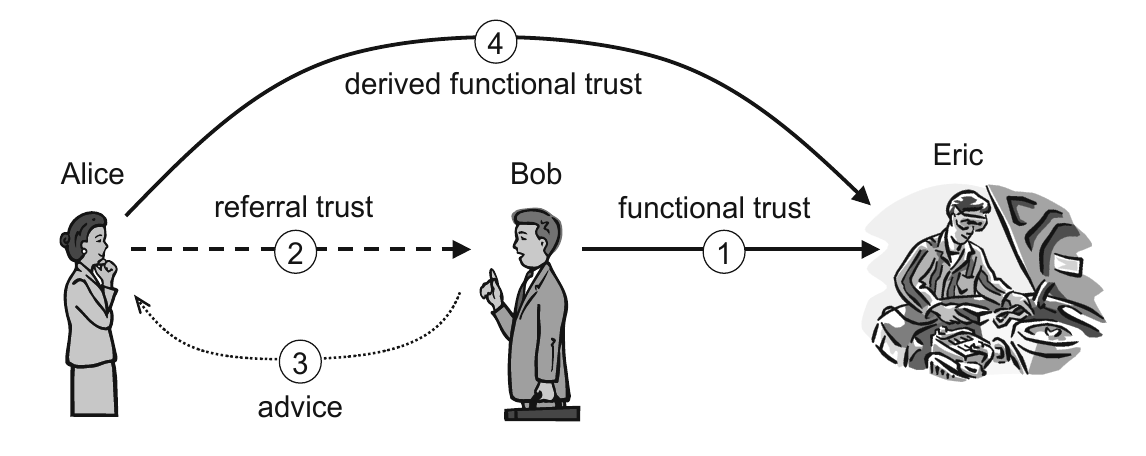
\includegraphics[scale=0.4]{images/transitive-trust-principle.png}
	\caption{Transitive trust principle}
\end{figure}

The trust that Alice has about Bob is called \emph{referral trust} and is denoted as $[A; B]$. The trust that Bob has about Erik is called \emph{functional trust} and is denoted as $[B, C]$. The trust that Alice has about Erik through Bob is called \emph{derived functional trust} as is denoted as:
\begin{equation}
	\begin{array}{rll}
		[A, E] & = [A; B] : [B, E] \\
		& = [A; B, E] \text{.} & \text{(Compact notation)}
	\end{array}
\end{equation}

Let $\opia{A}{B}$ be the trust opinion that Alice has about Bob, $\opia{B}{E}$ be the trust opinion that Bob has about Erik, and $\opia{[A;B]}{E}$ be the trust opinion that Alice has about Erik through Bob. We obtain the opinion $\opia{[A;B]}{E}$ by the operator trust discount and is defined below.

\begin{definition}
(\emph{Trust Discounting for Two-Edge Path}) Assume agents $A$ and $B$, where $A$ has referral trust in $B$ for a trust scope represented by domain $\dom{X}$. Let $X$ denote a variable on domain $X$, and let $\opia{B}{X} = (\bmda{B}{X}, \uax{B}{X}, \ada{B}{X}))$ be agent $B$’s general opinion on $X$ as advised by $B$ to $A$. Assume further that agent $A$’s referral trust in $B$, with respect to advising belief about $X$, is expressed as $\opia{A}{B}$. The notation for trust discount is given by
\begin{equation}
	\opia{[A;B]}{X} = \opia{A}{B} \otimes \opia{B}{X} \text{.}
\end{equation}

The trust-discounting operator combines agent $A$’s referral trust opinion about agent $B$, denoted $\opia{A}{B}$, to discount $B$’s opinion about variable $X$, denoted $\opia{B}{X}$, to produce $A$’s derived opinion about $X$, denoted $\opia{[A;B]}{X}$. The parameters of the derived opinion $\opia{[A;B]}{X}$ are defined in the following way:
\begin{equation}
	\opia{[A;B]}{X} = \left\{
	\begin{array}{ll}
		\bmdax{[A;B]}{X}{x} & = \ppa{A}{B} \bmdax{B}{X}{x} \text{,}\\
		\uax{[A;B]}{X} & = 1 - \ppa{A}{B} \sum\limits_{x \in \hdom{X}} \bmdax{B}{X}{x} \text{,} \\
		\adax{[A;B]}{X}{x} & = \adax{B}{X}{x} \text{.}
	\end{array}
	\right.
\end{equation}
\end{definition}

In particular, when $A$ fully trusts $B$, the opinion that $A$ has about $X$ will be completely accepted for $A$. Also, when $A$ fully distrusts $B$, then the opinion that $A$ has about $X$ will be completely rejected for $A$ and $A$ will have an opinion completely uncertain.

The previous example considers the relationship $[A, E]$ as a functional trust relationship. We also can consider as a belief relationship. Suppose now that Alice needs to go to a restaurant, but she doesn't know any restaurant in the town. Alice knows that Bob has good taste for restaurants and she asks him advice. Bob tells Alice about some restaurants to go to and his favorites.

Let $\dom{X}$ be the domain of all restaurants in town. Let $X$ be the variable over $\dom{X}$ that describes the best restaurant. The relationship $[A, X]$ is not about trust but belief. Bob acts as a \emph{source information} for Alice about $X$. Trust discounting also applies here.

\begin{figure}[htb]
	\centering
	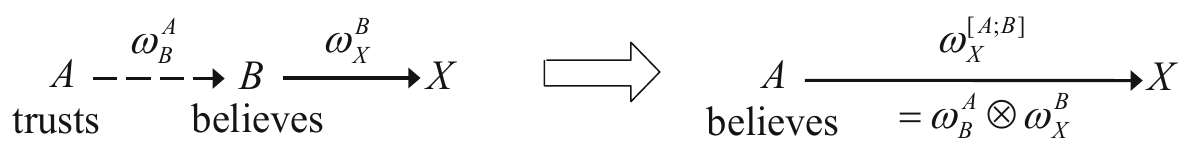
\includegraphics[scale=0.3]{images/trust-discounting-of-opinions.png}
	\caption{Trust discounting of opinions}
\end{figure}

\subsection{Trust fusion}

Suppose that Alice now wants the opinion of Clarie about the restaurants in town. She has different trust opinions about Bob and Clarie and she wants to consider both. Belief fusion $\oplus$ is the operator that solves that issue. I don't know the details about the operator yet, because there is a whole chapter for it. Here, I explain how it works with trust opinions.

We use the symbol $\diamond$ to denote a fusion between two relations:
\begin{equation}
	\begin{array}{rll}
		[A,E] & = ([A; B] : [B, X]) \diamond([A; C] : [C, X]) \\
		& = [A; B, C] \diamond [A; C, X] \text{.} & \text{(Compact notation)} 
	\end{array}
\end{equation}

The opinion that Alice has about X through the Bob and Clarie is:
\begin{equation}
	\opia{[A; B] \diamond [A; C]}{X} = (\opia{A}{B} \otimes \opia{B}{X}) \oplus (\opia{A}{C} \otimes \opia{C}{X})
\end{equation}

\begin{figure}[htb]
	\centering
	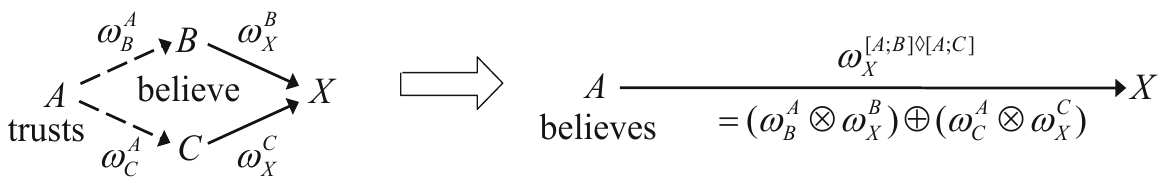
\includegraphics[scale=0.32]{images/fusion-of-trust-discounted-opinions.png}
	\caption{Fusion of trust-discounted opinions}
\end{figure}

%This is an overview. Nothing formal. (Maybe it will be if I have time.)
%
%\begin{itemize}
%	\item Definition of trust. (Influence?)
%	
%	\item Trust transitivity. (Update function?)
%	
%	\item Belief fusion. (Overall update function?)
%\end{itemize}

\section{The model and next questions}

We have a goal to improve or model with subjective logic. At first, I was thinking of model a society with the following representations:
\begin{itemize}
	\item The influence of an agent B over an agent A can be represented by the trust opinion $\opia{A}{B}$.
	
	\item Trust transitivity can be useful for update functions.
	
	\item When an agent has a trust opinion for each of the other agents of the society, trust fusion can be used to obtain the overall belief update.
\end{itemize}

The first problem is: \textbf{Trust discounting does not consider the case that the trustor already has an opinion}. Because of it, we don't have \emph{update}. To solve it, I plan to search if someone had the same problem before in the literature and search for some operator in subjective logic that has the same properties that we expect. If I don't find any operator, it may be the case of creating one, but I don't if this is \emph{allowed} in subjective logic.

The second problem is: \textbf{How to represent influence by a trust opinion?}. Suppose that an agent B has no influence on A ($I(A, B) = 0$). I thought of two ways to represent by an opinion: a) $\opia{A}{B} = (0, 0, 1, a^A_B)$), agent A is completely uncertain about trusting in B, or b) $\opia{A}{B} = (0, 1, 0, a^A_B)$, agent A completely distrusts B. I have to understand the difference between this representations when trust discounting and trust fusion are applied.

In this document, I presented what I find most useful for the research about group polarization in social networks. I studied some other topics that I didn't present here like the difference between aleatory and epistemic opinions, decision theory in subjective logic, and how opinions can be represented with Beta PDFs and Dirichlet PDFs.




%When I was reviewing the book, I found something that I may have got wrong about trust transitivity. I'm not sure if the example I told at the meeting is possible in SL.
%
%\begin{itemize}
%	\item Suppose that an agent A trusts an agent B ($\omega^A_B$), and B trusts X ($\omega^A_X$). Can the carnality of the domain of $\omega^A_X$ be greater than 2? (At the meeting, assumed yes. Now I'm not sure.)
%	
%	\item Is there a way (an operator) to consider the trust of an agent A when they obtain another trust opinion (from trust transitivity)?
%	
%	\begin{itemize}
%		\item If yes, can this operator have the same properties as the rational belief update?
%		
%		\item If not, can we create an operator that has the same properties as the rational belief update?
%	\end{itemize}
%\end{itemize}


%\bibliographystyle{plain}
%\bibliography{bibliography.bib}


\end{document}